\section{Spring Boot Gateway Implementation}

\subsection{Build Configuration}

\begin{lstlisting}[language=Kotlin, caption=build.gradle.kts]
plugins {
    kotlin("jvm") version "1.9.22"
    kotlin("plugin.spring") version "1.9.22"
    id("org.springframework.boot") version "3.2.4"
    id("io.spring.dependency-management") version "1.1.4"
    id("com.google.protobuf") version "0.9.4"
}

java {
    sourceCompatibility = JavaVersion.VERSION_17
}

repositories {
    mavenCentral()
}

dependencies {
    // Spring Boot Core
    implementation("org.springframework.boot:spring-boot-starter-webflux")
    implementation("org.springframework.boot:spring-boot-starter-actuator")

    // GraphQL
    implementation("org.springframework.boot:spring-boot-starter-graphql")

    // gRPC
    implementation("net.devh:grpc-spring-boot-starter:3.1.0.RELEASE")
    implementation("io.grpc:grpc-kotlin-stub:1.4.1")
    implementation("io.grpc:grpc-protobuf:1.60.1")
    implementation("com.google.protobuf:protobuf-kotlin:3.25.2")

    // Kotlin Coroutines
    implementation("org.jetbrains.kotlinx:kotlinx-coroutines-core:1.8.0")
    implementation("org.jetbrains.kotlinx:kotlinx-coroutines-reactor:1.8.0")
    implementation("io.projectreactor.kotlin:reactor-kotlin-extensions")

    // Hardware Access (Pi4J for SPI/GPIO)
    // Pi4J 2.6+ required for Raspberry Pi 5 (RP1 chip support via GpioD)
    implementation("com.pi4j:pi4j-core:2.6.1")
    implementation("com.pi4j:pi4j-plugin-raspberrypi:2.6.1")
    implementation("com.pi4j:pi4j-plugin-gpiod:2.6.1")  // Required for RPi5
    implementation("com.pi4j:pi4j-plugin-linuxfs:2.6.1")

    // Metrics
    implementation("io.micrometer:micrometer-registry-prometheus")

    // JSON Processing
    implementation("com.fasterxml.jackson.module:jackson-module-kotlin")

    // Kotlin Reflection
    implementation("org.jetbrains.kotlin:kotlin-reflect")

    // Testing
    testImplementation("org.springframework.boot:spring-boot-starter-test")
    testImplementation("io.projectreactor:reactor-test")
}

protobuf {
    protoc {
        artifact = "com.google.protobuf:protoc:3.25.2"
    }
    plugins {
        id("grpc") {
            artifact = "io.grpc:protoc-gen-grpc-java:1.60.1"
        }
        id("grpckt") {
            artifact = "io.grpc:protoc-gen-grpc-kotlin:1.4.1:jdk8@jar"
        }
    }
    generateProtoTasks {
        all().forEach {
            it.plugins {
                id("grpc")
                id("grpckt")
            }
            it.builtins {
                id("kotlin")
            }
        }
    }
}

tasks.withType<org.jetbrains.kotlin.gradle.tasks.KotlinCompile> {
    kotlinOptions {
        freeCompilerArgs += "-Xjsr305=strict"
        jvmTarget = "17"
    }
}
\end{lstlisting}

\subsection{Application Configuration}

\begin{lstlisting}[language=yaml, caption=application.yml]
spring:
  application:
    name: star-gateway
  graphql:
    graphiql:
      enabled: true
      path: /graphiql
    websocket:
      path: /graphql-ws
    schema:
      locations: classpath:graphql/
  main:
    banner-mode: off

server:
  port: 8080

grpc:
  server:
    port: 9090

# Hardware configuration
star:
  esp32:
    spi:
      enabled: true
      bus: 0
      chip-select: 0
      speed-hz: 10000000  # 10 MHz for motor control
      mode: 0
    tcp:
      enabled: true
      host: 192.168.4.2  # ESP32 IP on AP network
      port: 5000
      timeout-ms: 100
      retry-attempts: 3
  lidar:
    serial-port: /dev/ttyAMA0
    baud-rate: 460800
    protocol: SLAMTEC
    scan-rate-hz: 10

# Actuator endpoints for health checks
management:
  endpoints:
    web:
      exposure:
        include: health,prometheus,info,metrics
  endpoint:
    health:
      show-details: always
  metrics:
    tags:
      application: star-gateway

logging:
  level:
    com.star.gateway: DEBUG
    org.springframework.graphql: INFO
\end{lstlisting}

\subsection{Six-Layer Software Architecture}

The STAR system follows a strict six-layer architecture spanning from the remote UI to embedded firmware:

\begin{figure}[H]
\centering
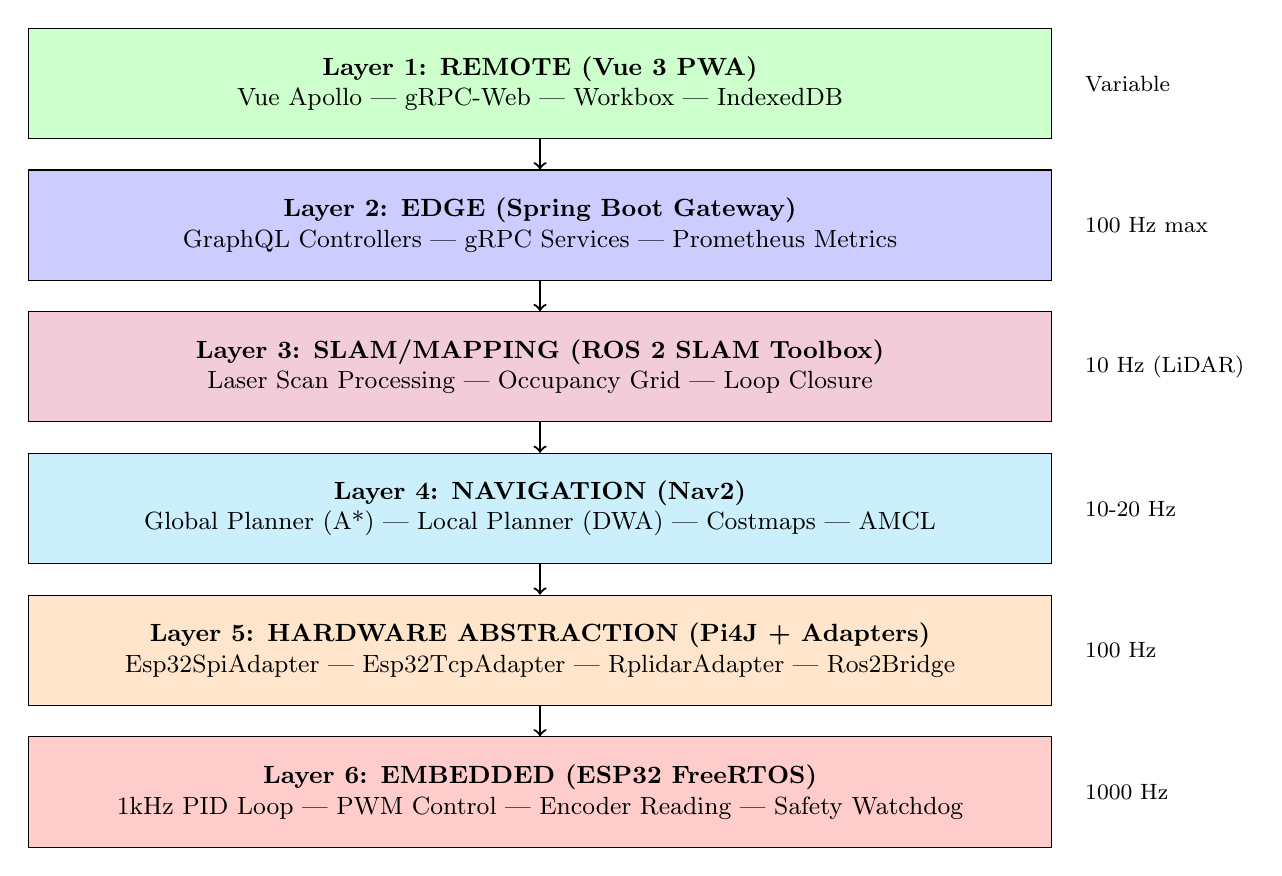
\begin{tikzpicture}[
    layer/.style={draw, rectangle, minimum width=13cm, minimum height=1.4cm, align=center, font=\small}
]
    % Layer 1: Remote
    \node[layer, fill=green!20] (remote) at (0,9) {
        \textbf{Layer 1: REMOTE (Vue 3 PWA)}\\
        Vue Apollo | gRPC-Web | Workbox | IndexedDB
    };

    % Layer 2: Edge
    \node[layer, fill=blue!20] (edge) at (0,7.2) {
        \textbf{Layer 2: EDGE (Spring Boot Gateway)}\\
        GraphQL Controllers | gRPC Services | Prometheus Metrics
    };

    % Layer 3: SLAM
    \node[layer, fill=purple!20] (slam) at (0,5.4) {
        \textbf{Layer 3: SLAM/MAPPING (ROS 2 SLAM Toolbox)}\\
        Laser Scan Processing | Occupancy Grid | Loop Closure
    };

    % Layer 4: Navigation
    \node[layer, fill=cyan!20] (nav) at (0,3.6) {
        \textbf{Layer 4: NAVIGATION (Nav2)}\\
        Global Planner (A*) | Local Planner (DWA) | Costmaps | AMCL
    };

    % Layer 5: Hardware Abstraction
    \node[layer, fill=orange!20] (hal) at (0,1.8) {
        \textbf{Layer 5: HARDWARE ABSTRACTION (Pi4J + Adapters)}\\
        Esp32SpiAdapter | Esp32TcpAdapter | RplidarAdapter | Ros2Bridge
    };

    % Layer 6: Embedded
    \node[layer, fill=red!20] (embedded) at (0,0) {
        \textbf{Layer 6: EMBEDDED (ESP32 FreeRTOS)}\\
        1kHz PID Loop | PWM Control | Encoder Reading | Safety Watchdog
    };

    % Arrows
    \draw[->, thick] (remote) -- (edge);
    \draw[->, thick] (edge) -- (slam);
    \draw[->, thick] (slam) -- (nav);
    \draw[->, thick] (nav) -- (hal);
    \draw[->, thick] (hal) -- (embedded);

    % Update rates on the right
    \node[right, font=\footnotesize] at (6.8,9) {Variable};
    \node[right, font=\footnotesize] at (6.8,7.2) {100 Hz max};
    \node[right, font=\footnotesize] at (6.8,5.4) {10 Hz (LiDAR)};
    \node[right, font=\footnotesize] at (6.8,3.6) {10-20 Hz};
    \node[right, font=\footnotesize] at (6.8,1.8) {100 Hz};
    \node[right, font=\footnotesize] at (6.8,0) {1000 Hz};

\end{tikzpicture}
\caption{Six-Layer Software Architecture with Update Frequencies}
\end{figure}

\subsubsection{Layer Responsibilities}

\begin{description}[style=nextline, leftmargin=1cm]
    \item[Layer 1 - Remote (Vue 3 PWA)] User interface running in browser or as installed PWA. Handles user input, displays telemetry, provides offline capability via service workers and IndexedDB.

    \item[Layer 2 - Edge (Spring Boot Gateway)] API gateway running on RPi5. Translates between web protocols (GraphQL/gRPC) and robot internals. Manages authentication, rate limiting, and metrics.

    \item[Layer 3 - SLAM/Mapping (ROS 2 SLAM Toolbox)] Processes LiDAR scans to build occupancy grid maps. Handles loop closure detection and map optimization. Updates at LiDAR scan rate (10 Hz).

    \item[Layer 4 - Navigation (Nav2)] Path planning and obstacle avoidance. Global planner (A*) runs at 10 Hz, local planner (DWA) runs at 20 Hz. Publishes velocity commands to Layer 5.

    \item[Layer 5 - Hardware Abstraction (Pi4J + Adapters)] Interfaces between ROS 2 and physical hardware. Communicates with ESP32 via SPI (primary) and TCP (fallback). Reads LiDAR via UART (rplidar\_ros2 driver).

    \item[Layer 6 - Embedded (ESP32 FreeRTOS)] Real-time motor control at 1 kHz. Runs PID loops, reads encoders, generates PWM signals. Maintains safe operation even if higher layers fail.
\end{description}

\subsubsection{Control Timing Hierarchy}

The STAR robot operates with a multi-rate control hierarchy, where each layer runs at a frequency appropriate to its function:

\begin{figure}[H]
\centering
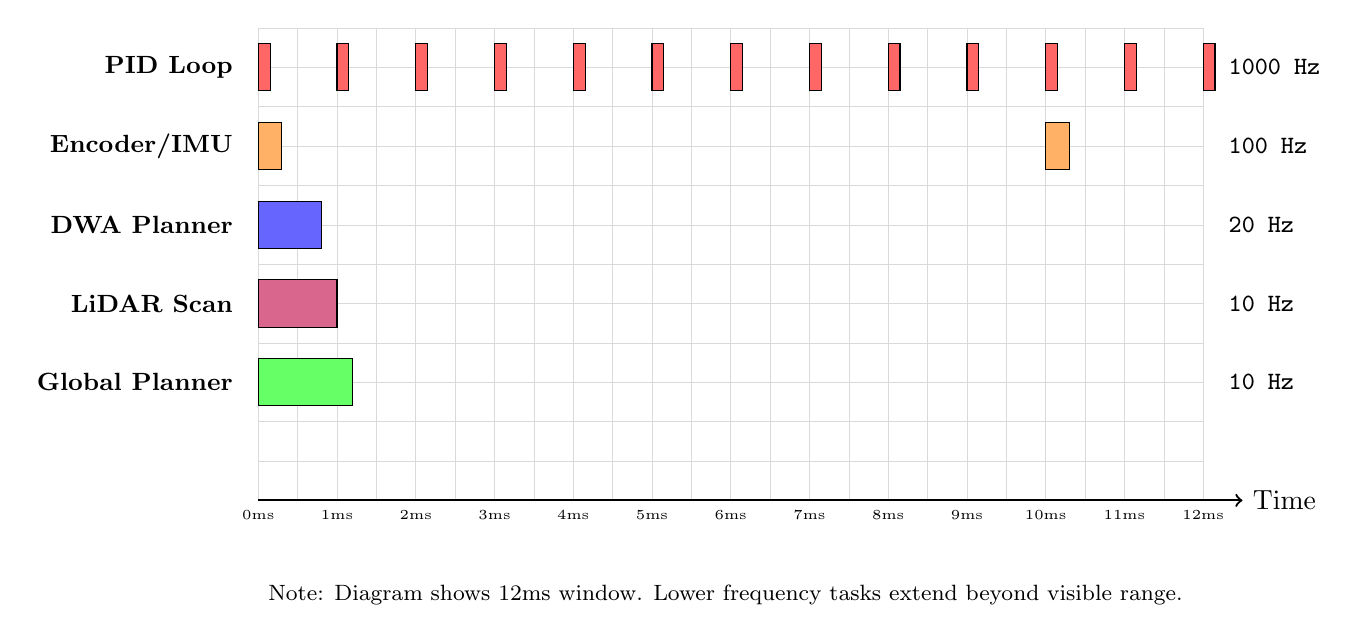
\begin{tikzpicture}[
    timebar/.style={draw, rectangle, minimum height=0.8cm, fill=#1},
    label/.style={font=\small\bfseries},
    freq/.style={font=\small\ttfamily}
]
    % Background grid showing time
    \draw[gray!30, very thin] (0,0) grid[step=0.5] (12,6);

    % Time axis
    \draw[->, thick] (0,0) -- (12.5,0) node[right] {Time};
    \foreach \x in {0,1,2,3,4,5,6,7,8,9,10,11,12} {
        \node[below, font=\tiny] at (\x,0) {\x ms};
    }

    % 1000 Hz PID Loop (ESP32) - every 1ms
    \foreach \x in {0,1,2,3,4,5,6,7,8,9,10,11,12} {
        \draw[fill=red!60] (\x,5.2) rectangle (\x+0.15,5.8);
    }
    \node[label, left] at (-0.2,5.5) {PID Loop};
    \node[freq, right] at (12.2,5.5) {1000 Hz};

    % 100 Hz Encoder/IMU (ESP32) - every 10ms
    \foreach \x in {0,10} {
        \draw[fill=orange!60] (\x,4.2) rectangle (\x+0.3,4.8);
    }
    \node[label, left] at (-0.2,4.5) {Encoder/IMU};
    \node[freq, right] at (12.2,4.5) {100 Hz};

    % 20 Hz DWA Local Planner - every 50ms (not visible in 12ms window, show one)
    \draw[fill=blue!60] (0,3.2) rectangle (0.8,3.8);
    \node[label, left] at (-0.2,3.5) {DWA Planner};
    \node[freq, right] at (12.2,3.5) {20 Hz};

    % 10 Hz LiDAR Scan - every 100ms (not visible in 12ms window, show one)
    \draw[fill=purple!60] (0,2.2) rectangle (1.0,2.8);
    \node[label, left] at (-0.2,2.5) {LiDAR Scan};
    \node[freq, right] at (12.2,2.5) {10 Hz};

    % 10 Hz Global Planner - every 100ms (not visible in 12ms window, show one)
    \draw[fill=green!60] (0,1.2) rectangle (1.2,1.8);
    \node[label, left] at (-0.2,1.5) {Global Planner};
    \node[freq, right] at (12.2,1.5) {10 Hz};

    % Legend
    \node[align=left, font=\footnotesize] at (6,-1.2) {
        Note: Diagram shows 12ms window. Lower frequency tasks extend beyond visible range.
    };

\end{tikzpicture}
\caption{Control Timing Hierarchy (12ms Window)}
\end{figure}

\begin{table}[H]
\centering
\caption{Control Loop Frequencies and Responsibilities}
\begin{tabular}{|l|c|l|l|}
\hline
\textbf{Control Loop} & \textbf{Frequency} & \textbf{Period} & \textbf{Processor} \\
\hline
PID Motor Control & 1000 Hz & 1 ms & ESP32 (FreeRTOS) \\
\hline
Encoder/IMU Sampling & 100 Hz & 10 ms & ESP32 (FreeRTOS) \\
\hline
DWA Local Planner & 20 Hz & 50 ms & RPi5 (Nav2) \\
\hline
LiDAR Scan Processing & 10 Hz & 100 ms & RPi5 (ROS 2) \\
\hline
Global Path Planner & 10 Hz & 100 ms & RPi5 (Nav2) \\
\hline
Telemetry Publishing & 10 Hz & 100 ms & RPi5 (Spring Boot) \\
\hline
Map Updates & 2 Hz & 500 ms & RPi5 (SLAM Toolbox) \\
\hline
\end{tabular}
\end{table}

\textbf{Timing Design Rationale}:
\begin{itemize}
    \item \textbf{1000 Hz PID} -- Required for smooth motor control and quick response to disturbances. FreeRTOS ensures deterministic timing.

    \item \textbf{100 Hz Sensor Sampling} -- Captures high-frequency vibrations and provides accurate velocity estimates via differentiation.

    \item \textbf{20 Hz DWA} -- Fast enough for obstacle avoidance at max velocity (0.5 m/s = 2.5cm per cycle), slow enough to not overload CPU.

    \item \textbf{10 Hz LiDAR} -- Fixed by RPLiDAR C1 hardware. Sufficient for indoor navigation at walking speeds.

    \item \textbf{10 Hz Global Planner} -- Path replanning happens infrequently; 10 Hz allows quick re-routing while minimizing CPU load.
\end{itemize}

\subsection{GraphQL Schema}

\begin{lstlisting}[language=GraphQL, caption=schema.graphqls]
# Query operations - read-only data fetching
type Query {
    telemetry: Telemetry!
    systemStatus: SystemStatus!
    settings: Settings!
    navigationState: NavigationState!
    telemetryHistory(limit: Int = 100): [TelemetrySnapshot!]!
}

# Mutation operations - state changes
type Mutation {
    setMode(mode: RobotMode!): Boolean!
    emergencyStop: Boolean!
    setSettings(input: SettingsInput!): Settings!
    addWaypoint(x: Float!, y: Float!): Waypoint!
    clearWaypoints: Boolean!
    startNavigation: Boolean!
    stopNavigation: Boolean!
}

# Subscription operations - real-time streams
type Subscription {
    telemetryStream: Telemetry!
    lidarScan: LidarScan!
    eventLog: Event!
}

# Core telemetry data structure
type Telemetry {
    imu: ImuData!
    gps: GpsData!
    battery: Float!
    wifiSignal: Int!
    cpuUsage: Float!
    temperature: Float!
    motorLoad: Float!
    timestamp: String!
}

type ImuData {
    pitch: Float!
    roll: Float!
    yaw: Float!
    velocity: Float!
    accelerationX: Float!
    accelerationY: Float!
    accelerationZ: Float!
}

type GpsData {
    latitude: Float!
    longitude: Float!
    altitude: Float!
}

type LidarScan {
    points: [LidarPoint!]!
    timestamp: String!
}

type LidarPoint {
    angle: Float!
    distance: Float!
    intensity: Float!
}

type SystemStatus {
    connectionStatus: ConnectionStatus!
    mode: RobotMode!
    esp32Connected: Boolean!
    lidarConnected: Boolean!
    rosConnected: Boolean!
}

type NavigationState {
    currentPosition: Position!
    path: [Position!]!
    waypoints: [Waypoint!]!
    isNavigating: Boolean!
}

type Position {
    x: Float!
    y: Float!
    heading: Float!
}

type Waypoint {
    id: ID!
    x: Float!
    y: Float!
    label: String
}

type Event {
    timestamp: String!
    message: String!
    type: EventType!
}

type Settings {
    maxSpeed: Float!
    safetyLockEnabled: Boolean!
    autonomousEnabled: Boolean!
    lidarEnabled: Boolean!
}

input SettingsInput {
    maxSpeed: Float
    safetyLockEnabled: Boolean
    autonomousEnabled: Boolean
    lidarEnabled: Boolean
}

enum RobotMode {
    IDLE
    MANUAL
    AUTONOMOUS
    MAPPING
    EMERGENCY_STOP
}

enum ConnectionStatus {
    CONNECTED
    DISCONNECTED
    CONNECTING
    ERROR
}

enum EventType {
    INFO
    SUCCESS
    WARNING
    ERROR
}
\end{lstlisting}

\subsection{gRPC Protobuf Definition}

\begin{lstlisting}[language=Protobuf, caption=motor\_control.proto]
syntax = "proto3";

package star.motor;

option java_package = "com.star.gateway.proto";
option java_outer_classname = "MotorControlProto";
option java_multiple_files = true;

// Motor control service for low-latency commands
service MotorControl {
    // Unary RPCs (single request-response)
    rpc SetVelocity(VelocityCommand) returns (CommandResponse);
    rpc EmergencyStop(EmptyRequest) returns (CommandResponse);
    rpc SetMotorPower(MotorPowerCommand) returns (CommandResponse);

    // Server streaming (continuous encoder feedback)
    rpc StreamEncoderData(EmptyRequest) returns (stream EncoderData);
}

// Velocity command for differential drive
message VelocityCommand {
    float left_velocity = 1;   // m/s, range: -2.0 to 2.0
    float right_velocity = 2;  // m/s, range: -2.0 to 2.0
    uint64 timestamp = 3;      // Unix timestamp in milliseconds
}

// Direct motor power control
message MotorPowerCommand {
    int32 motor_id = 1;        // Motor index: 0-3
    float power = 2;           // Power level: -1.0 to 1.0
}

// Standard command response
message CommandResponse {
    bool success = 1;          // True if command executed
    string message = 2;        // Human-readable status
    uint64 latency_us = 3;     // Round-trip latency in microseconds
}

// Real-time encoder data
message EncoderData {
    int32 motor_id = 1;        // Motor index: 0-3
    int64 ticks = 2;           // Absolute encoder position
    float velocity = 3;        // Current velocity in m/s
    uint64 timestamp = 4;      // Unix timestamp in milliseconds
}

// Empty request placeholder
message EmptyRequest {}
\end{lstlisting}

\subsection{Service Implementations}

\subsubsection{Motor Control Service}

\begin{lstlisting}[language=Kotlin, caption=MotorControlService.kt]
package com.star.gateway.service

import com.star.gateway.hardware.Esp32SpiAdapter
import com.star.gateway.hardware.Esp32TcpAdapter
import com.star.gateway.model.CommandResult
import io.micrometer.core.instrument.MeterRegistry
import io.micrometer.core.instrument.Timer
import kotlinx.coroutines.async
import kotlinx.coroutines.coroutineScope
import org.slf4j.LoggerFactory
import org.springframework.stereotype.Service
import java.util.concurrent.TimeUnit

@Service
class MotorControlService(
    private val esp32SpiAdapter: Esp32SpiAdapter,
    private val esp32TcpAdapter: Esp32TcpAdapter,
    private val meterRegistry: MeterRegistry
) {
    private val logger = LoggerFactory.getLogger(javaClass)

    // Metrics
    private val commandCounter = meterRegistry.counter("motor.commands.total")
    private val spiErrorCounter = meterRegistry.counter("motor.spi.errors")
    private val tcpFallbackCounter = meterRegistry.counter("motor.tcp.fallbacks")
    private val latencyTimer: Timer = Timer.builder("motor.command.latency")
        .description("Motor command round-trip latency")
        .register(meterRegistry)

    /**
     * Send velocity command to ESP32.
     * Primary: SPI (lowest latency)
     * Fallback: TCP (if SPI fails)
     */
    suspend fun setVelocity(left: Float, right: Float): CommandResult {
        val startTime = System.nanoTime()

        return try {
            val result = esp32SpiAdapter.sendVelocityCommand(left, right)
            commandCounter.increment()
            latencyTimer.record(System.nanoTime() - startTime, TimeUnit.NANOSECONDS)
            result
        } catch (e: Exception) {
            logger.warn("SPI failed, falling back to TCP: ${e.message}")
            spiErrorCounter.increment()
            tcpFallbackCounter.increment()

            try {
                esp32TcpAdapter.sendVelocityCommand(left, right)
            } catch (tcpException: Exception) {
                logger.error("TCP fallback also failed: ${tcpException.message}")
                CommandResult.failure("Both SPI and TCP communication failed")
            }
        }
    }

    /**
     * Emergency stop - send to BOTH channels simultaneously for redundancy.
     * Returns success if either channel succeeds.
     */
    suspend fun emergencyStop(): CommandResult {
        logger.warn("EMERGENCY STOP triggered")

        return coroutineScope {
            val spiDeferred = async {
                runCatching { esp32SpiAdapter.emergencyStop() }
            }
            val tcpDeferred = async {
                runCatching { esp32TcpAdapter.emergencyStop() }
            }

            val spiResult = spiDeferred.await()
            val tcpResult = tcpDeferred.await()

            when {
                spiResult.isSuccess && tcpResult.isSuccess -> {
                    logger.info("Emergency stop confirmed on both channels")
                    CommandResult.success("Emergency stop executed on both channels")
                }
                spiResult.isSuccess || tcpResult.isSuccess -> {
                    logger.warn("Emergency stop partially successful")
                    CommandResult.success("Emergency stop executed (partial)")
                }
                else -> {
                    logger.error("Emergency stop FAILED on both channels!")
                    CommandResult.failure("Emergency stop failed on both channels")
                }
            }
        }
    }

    /**
     * Get current connection status for both channels.
     */
    fun getConnectionStatus(): Map<String, Boolean> {
        return mapOf(
            "spi" to esp32SpiAdapter.isConnected(),
            "tcp" to esp32TcpAdapter.isConnected()
        )
    }
}
\end{lstlisting}

\subsubsection{ESP32 SPI Adapter}

\begin{lstlisting}[language=Kotlin, caption=Esp32SpiAdapter.kt]
package com.star.gateway.hardware

import com.pi4j.Pi4J
import com.pi4j.context.Context
import com.pi4j.io.spi.Spi
import com.pi4j.io.spi.SpiMode
import com.star.gateway.model.CommandResult
import org.slf4j.LoggerFactory
import org.springframework.beans.factory.annotation.Value
import org.springframework.stereotype.Component
import java.nio.ByteBuffer
import java.nio.ByteOrder
import javax.annotation.PostConstruct
import javax.annotation.PreDestroy

@Component
class Esp32SpiAdapter(
    @Value("\${star.esp32.spi.enabled:true}")
    private val enabled: Boolean,

    @Value("\${star.esp32.spi.bus:0}")
    private val spiBus: Int,

    @Value("\${star.esp32.spi.chip-select:0}")
    private val chipSelect: Int,

    @Value("\${star.esp32.spi.speed-hz:10000000}")  // 10 MHz default
    private val speedHz: Int,

    @Value("\${star.esp32.spi.mode:0}")
    private val spiModeValue: Int
) {
    private val logger = LoggerFactory.getLogger(javaClass)

    private var pi4j: Context? = null
    private var spi: Spi? = null
    private var connected = false

    // SPI Command bytes
    companion object {
        const val CMD_SET_VELOCITY: Byte = 0x01
        const val CMD_EMERGENCY_STOP: Byte = 0x02
        const val CMD_GET_ENCODERS: Byte = 0x03
        const val CMD_SET_MOTOR: Byte = 0x04
        const val CMD_PING: Byte = 0x05

        const val RESPONSE_OK: Byte = 0x00
        const val RESPONSE_ERROR: Byte = 0x01
    }

    @PostConstruct
    fun initialize() {
        if (!enabled) {
            logger.info("SPI adapter disabled by configuration")
            return
        }

        try {
            pi4j = Pi4J.newAutoContext()

            val spiConfig = Spi.newConfigBuilder(pi4j)
                .id("esp32-spi")
                .name("ESP32 Motor Controller")
                .bus(spiBus)
                .chipSelect(chipSelect)
                .baud(speedHz)
                .mode(SpiMode.entries[spiModeValue])
                .build()

            spi = pi4j?.create(spiConfig)
            connected = testConnection()

            logger.info("SPI adapter initialized: bus=$spiBus, cs=$chipSelect, speed=$speedHz Hz")
        } catch (e: Exception) {
            logger.error("Failed to initialize SPI adapter: ${e.message}")
            connected = false
        }
    }

    @PreDestroy
    fun shutdown() {
        spi?.close()
        pi4j?.shutdown()
        logger.info("SPI adapter shutdown complete")
    }

    /**
     * Send velocity command.
     * Packet format: [CMD_SET_VELOCITY (1), left_velocity (4), right_velocity (4)]
     * Response: [status (1)]
     */
    suspend fun sendVelocityCommand(left: Float, right: Float): CommandResult {
        if (!enabled || spi == null) {
            throw IllegalStateException("SPI not initialized")
        }

        val buffer = ByteBuffer.allocate(9)
            .order(ByteOrder.LITTLE_ENDIAN)
            .put(CMD_SET_VELOCITY)
            .putFloat(left)
            .putFloat(right)

        val txData = buffer.array()
        val rxData = ByteArray(2)

        synchronized(this) {
            spi!!.transfer(txData, rxData)
        }

        return if (rxData[0] == RESPONSE_OK) {
            CommandResult.success("Velocity set: left=$left, right=$right")
        } else {
            CommandResult.failure("ESP32 error code: ${rxData[0]}")
        }
    }

    /**
     * Send emergency stop command.
     * Packet format: [CMD_EMERGENCY_STOP (1)]
     * Response: [status (1)]
     */
    suspend fun emergencyStop(): CommandResult {
        if (!enabled || spi == null) {
            throw IllegalStateException("SPI not initialized")
        }

        val txData = byteArrayOf(CMD_EMERGENCY_STOP)
        val rxData = ByteArray(2)

        synchronized(this) {
            spi!!.transfer(txData, rxData)
        }

        return if (rxData[0] == RESPONSE_OK) {
            CommandResult.success("Emergency stop executed")
        } else {
            CommandResult.failure("Emergency stop failed: ${rxData[0]}")
        }
    }

    /**
     * Test SPI connection with ping command.
     */
    private fun testConnection(): Boolean {
        return try {
            val txData = byteArrayOf(CMD_PING)
            val rxData = ByteArray(2)
            spi?.transfer(txData, rxData)
            rxData[0] == RESPONSE_OK
        } catch (e: Exception) {
            logger.warn("SPI connection test failed: ${e.message}")
            false
        }
    }

    fun isConnected(): Boolean = connected && enabled
}
\end{lstlisting}

\subsubsection{ESP32 TCP Adapter}

\begin{lstlisting}[language=Kotlin, caption=Esp32TcpAdapter.kt]
package com.star.gateway.hardware

import com.fasterxml.jackson.databind.ObjectMapper
import com.star.gateway.model.CommandResult
import kotlinx.coroutines.Dispatchers
import kotlinx.coroutines.withContext
import kotlinx.coroutines.withTimeoutOrNull
import org.slf4j.LoggerFactory
import org.springframework.beans.factory.annotation.Value
import org.springframework.stereotype.Component
import java.io.BufferedReader
import java.io.InputStreamReader
import java.io.PrintWriter
import java.net.InetSocketAddress
import java.net.Socket

@Component
class Esp32TcpAdapter(
    @Value("\${star.esp32.tcp.enabled:true}")
    private val enabled: Boolean,

    @Value("\${star.esp32.tcp.host:192.168.4.2}")
    private val host: String,

    @Value("\${star.esp32.tcp.port:5000}")
    private val port: Int,

    @Value("\${star.esp32.tcp.timeout-ms:100}")
    private val timeoutMs: Long,

    @Value("\${star.esp32.tcp.retry-attempts:3}")
    private val retryAttempts: Int,

    private val objectMapper: ObjectMapper
) {
    private val logger = LoggerFactory.getLogger(javaClass)

    data class TcpCommand(
        val command: String,
        val params: Map<String, Any> = emptyMap(),
        val timestamp: Long = System.currentTimeMillis()
    )

    data class TcpResponse(
        val success: Boolean,
        val message: String,
        val data: Map<String, Any>? = null
    )

    /**
     * Send velocity command via TCP.
     */
    suspend fun sendVelocityCommand(left: Float, right: Float): CommandResult {
        val command = TcpCommand(
            command = "velocity",
            params = mapOf(
                "left" to left,
                "right" to right
            )
        )
        return sendCommand(command)
    }

    /**
     * Send emergency stop via TCP.
     */
    suspend fun emergencyStop(): CommandResult {
        val command = TcpCommand(command = "emergency_stop")
        return sendCommand(command)
    }

    /**
     * Generic command sender with retry logic.
     */
    private suspend fun sendCommand(command: TcpCommand): CommandResult {
        if (!enabled) {
            return CommandResult.failure("TCP adapter disabled")
        }

        var lastException: Exception? = null

        repeat(retryAttempts) { attempt ->
            try {
                return withContext(Dispatchers.IO) {
                    withTimeoutOrNull(timeoutMs) {
                        executeCommand(command)
                    } ?: CommandResult.failure("TCP timeout after ${timeoutMs}ms")
                }
            } catch (e: Exception) {
                lastException = e
                logger.warn("TCP attempt ${attempt + 1}/$retryAttempts failed: ${e.message}")
            }
        }

        return CommandResult.failure(
            "TCP failed after $retryAttempts attempts: ${lastException?.message}"
        )
    }

    private fun executeCommand(command: TcpCommand): CommandResult {
        Socket().use { socket ->
            socket.connect(InetSocketAddress(host, port), timeoutMs.toInt())
            socket.soTimeout = timeoutMs.toInt()

            val writer = PrintWriter(socket.getOutputStream(), true)
            val reader = BufferedReader(InputStreamReader(socket.getInputStream()))

            // Send JSON command
            val json = objectMapper.writeValueAsString(command)
            writer.println(json)

            // Read response
            val responseLine = reader.readLine()
            val response = objectMapper.readValue(responseLine, TcpResponse::class.java)

            return if (response.success) {
                CommandResult.success(response.message)
            } else {
                CommandResult.failure(response.message)
            }
        }
    }

    /**
     * Check TCP connectivity.
     */
    fun isConnected(): Boolean {
        if (!enabled) return false

        return try {
            Socket().use { socket ->
                socket.connect(InetSocketAddress(host, port), timeoutMs.toInt())
                true
            }
        } catch (e: Exception) {
            false
        }
    }
}
\end{lstlisting}

\subsubsection{GraphQL Controller}

\begin{lstlisting}[language=Kotlin, caption=TelemetryController.kt]
package com.star.gateway.graphql

import com.star.gateway.model.*
import com.star.gateway.service.TelemetryService
import com.star.gateway.service.MotorControlService
import kotlinx.coroutines.flow.Flow
import org.springframework.graphql.data.method.annotation.Argument
import org.springframework.graphql.data.method.annotation.MutationMapping
import org.springframework.graphql.data.method.annotation.QueryMapping
import org.springframework.graphql.data.method.annotation.SubscriptionMapping
import org.springframework.stereotype.Controller
import reactor.core.publisher.Flux

@Controller
class TelemetryController(
    private val telemetryService: TelemetryService,
    private val motorControlService: MotorControlService
) {
    // ========== QUERIES ==========

    @QueryMapping
    suspend fun telemetry(): Telemetry {
        return telemetryService.getCurrentTelemetry()
    }

    @QueryMapping
    suspend fun systemStatus(): SystemStatus {
        return telemetryService.getSystemStatus()
    }

    @QueryMapping
    suspend fun telemetryHistory(
        @Argument limit: Int?
    ): List<TelemetrySnapshot> {
        return telemetryService.getHistory(limit ?: 100)
    }

    // ========== MUTATIONS ==========

    @MutationMapping
    suspend fun emergencyStop(): Boolean {
        val result = motorControlService.emergencyStop()
        return result.success
    }

    @MutationMapping
    suspend fun setMode(@Argument mode: RobotMode): Boolean {
        return telemetryService.setMode(mode)
    }

    // ========== SUBSCRIPTIONS ==========

    @SubscriptionMapping
    fun telemetryStream(): Flux<Telemetry> {
        return telemetryService.telemetryFlow()
            .asFlux()
    }

    @SubscriptionMapping
    fun eventLog(): Flux<Event> {
        return telemetryService.eventFlow()
            .asFlux()
    }
}

// Extension function to convert Flow to Flux
private fun <T> Flow<T>.asFlux(): Flux<T> {
    return kotlinx.coroutines.reactor.asFlux(this)
}
\end{lstlisting}

\subsubsection{gRPC Service}

\begin{lstlisting}[language=Kotlin, caption=MotorControlGrpcService.kt]
package com.star.gateway.grpc

import com.star.gateway.proto.*
import com.star.gateway.service.MotorControlService
import io.grpc.stub.StreamObserver
import kotlinx.coroutines.flow.Flow
import kotlinx.coroutines.flow.flow
import kotlinx.coroutines.runBlocking
import net.devh.boot.grpc.server.service.GrpcService
import org.slf4j.LoggerFactory

@GrpcService
class MotorControlGrpcService(
    private val motorControlService: MotorControlService
) : MotorControlGrpcKt.MotorControlCoroutineImplBase() {

    private val logger = LoggerFactory.getLogger(javaClass)

    /**
     * Handle velocity command via gRPC.
     */
    override suspend fun setVelocity(request: VelocityCommand): CommandResponse {
        val startTime = System.nanoTime()

        logger.debug("gRPC SetVelocity: left=${request.leftVelocity}, right=${request.rightVelocity}")

        val result = motorControlService.setVelocity(
            left = request.leftVelocity,
            right = request.rightVelocity
        )

        val latencyUs = (System.nanoTime() - startTime) / 1000

        return CommandResponse.newBuilder()
            .setSuccess(result.success)
            .setMessage(result.message)
            .setLatencyUs(latencyUs)
            .build()
    }

    /**
     * Handle emergency stop via gRPC.
     */
    override suspend fun emergencyStop(request: EmptyRequest): CommandResponse {
        logger.warn("gRPC EmergencyStop received")

        val result = motorControlService.emergencyStop()

        return CommandResponse.newBuilder()
            .setSuccess(result.success)
            .setMessage(result.message)
            .build()
    }

    /**
     * Stream encoder data to client.
     */
    override fun streamEncoderData(request: EmptyRequest): Flow<EncoderData> = flow {
        // Emit encoder data at 100Hz
        while (true) {
            val encoders = motorControlService.getEncoderData()

            encoders.forEach { (motorId, data) ->
                emit(
                    EncoderData.newBuilder()
                        .setMotorId(motorId)
                        .setTicks(data.ticks)
                        .setVelocity(data.velocity)
                        .setTimestamp(System.currentTimeMillis())
                        .build()
                )
            }

            kotlinx.coroutines.delay(10) // 100Hz
        }
    }
}
\end{lstlisting}

